\documentclass[tikz,border=0pt]{standalone}
% Shared publication style. Compile figure sources from this directory.
\usepackage[T1]{fontenc}
\usepackage{lmodern}
\usepackage{amsmath,amssymb}
\usepackage{tikz}
\usepackage{pgfplots}
\usetikzlibrary{arrows.meta,calc,positioning,backgrounds,patterns,shapes.geometric}
\usepgfplotslibrary{groupplots,fillbetween}
\pgfplotsset{compat=1.18}
\definecolor{fgblue}{HTML}{0072B2}
\definecolor{fgorange}{HTML}{D55E00}
\definecolor{fgslate}{HTML}{8B949E}
\definecolor{fgdark}{HTML}{25313C}
\definecolor{fgpale}{HTML}{F2F6F8}
\definecolor{fggrid}{HTML}{E3E8EC}
\definecolor{fgwater}{HTML}{D6EAF4}
\definecolor{fgland}{HTML}{E8E3D3}
\renewcommand{\familydefault}{\sfdefault}
\tikzset{every picture/.style={font=\fontsize{9}{11}\selectfont,text=fgdark},
  panel label/.style={font=\bfseries\fontsize{10}{12}\selectfont,anchor=north west},
  panel title/.style={font=\bfseries\fontsize{9}{11}\selectfont,anchor=north west},
  light arrow/.style={-{Stealth[length=1.6mm]},draw=fgslate,line width=.65pt}}
\pgfplotsset{fg axis/.style={
  axis line style={fgslate,line width=.4pt},axis x line*=bottom,axis y line*=left,
  tick align=outside,tick style={fgslate,line width=.4pt},
  tick label style={font=\fontsize{8}{10}\selectfont,text=fgdark},
  label style={font=\fontsize{9}{11}\selectfont,text=fgdark},
  title style={font=\bfseries\fontsize{9}{11}\selectfont,text=fgdark},
  grid style={fggrid,line width=.35pt},minor tick num=0,
  legend style={draw=none,fill=none,font=\fontsize{8}{10}\selectfont},
  scaled ticks=false,clip=false,
  every axis plot/.append style={line width=.85pt,mark size=2.2pt}
}}

% Source: reports/prospective_nuisance_shift_report_v2_rerun.md, tables 1--3.
% Every interval is the reported mean +/- 1.96*SE across five seeds, 22--26.
% Proportions multiplied by 100; no intervals reconstructed from arm contrasts.
\begin{document}
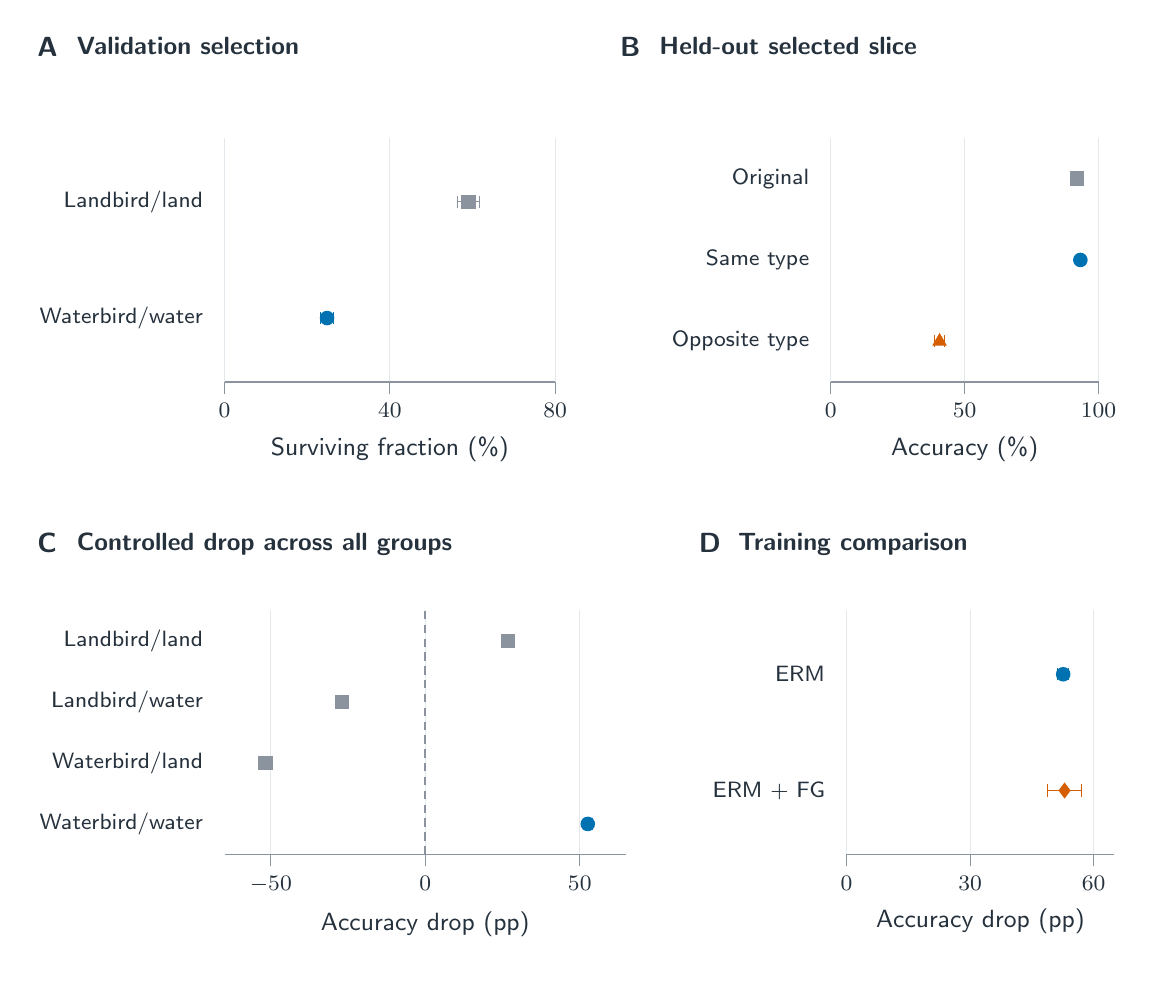
\begin{tikzpicture}[x=1mm,y=1mm]
\path[use as bounding box] (0,0) rectangle (140,119);
\node[panel label] at (0,119) {A};
\node[panel title] at (5,119) {Validation selection};
\node[panel label] at (74,119) {B};
\node[panel title] at (79,119) {Held-out selected slice};
\begin{axis}[fg axis,at={(25mm,74mm)},anchor=south west,width=42mm,height=31mm,scale only axis,
 xmin=0,xmax=80,xtick={0,40,80},ymin=.45,ymax=2.55,ytick={1,2},
 yticklabels={Waterbird/water,Landbird/land},yticklabel style={font=\fontsize{8}{10}\selectfont},
 xlabel={Surviving fraction (\%)},xmajorgrids=true,y axis line style={draw=none},ytick style={draw=none}]
\addplot[only marks,fgslate,mark=square*,error bars/.cd,x dir=both,x explicit]
 coordinates {(59,2) +- (2.7,0)};
\addplot[only marks,fgblue,mark=*,error bars/.cd,x dir=both,x explicit]
 coordinates {(24.8,1) +- (1.5,0)};
\end{axis}
\begin{axis}[fg axis,at={(102mm,74mm)},anchor=south west,width=34mm,height=31mm,scale only axis,
 xmin=0,xmax=100,xtick={0,50,100},ymin=.5,ymax=3.5,ytick={1,2,3},
 yticklabels={Opposite type,Same type,Original},
 xlabel={Accuracy (\%)},xmajorgrids=true,y axis line style={draw=none},ytick style={draw=none}]
\addplot[only marks,fgslate,mark=square*,error bars/.cd,x dir=both,x explicit]
 coordinates {(91.99,3) +- (.62,0)};
\addplot[only marks,fgblue,mark=*,error bars/.cd,x dir=both,x explicit]
 coordinates {(93.21,2) +- (.72,0)};
\addplot[only marks,fgorange,mark=triangle*,error bars/.cd,x dir=both,x explicit]
 coordinates {(40.62,1) +- (1.98,0)};
\end{axis}
\node[panel label] at (0,56) {C};
\node[panel title] at (5,56) {Controlled drop across all groups};
\node[panel label] at (84,56) {D};
\node[panel title] at (89,56) {Training comparison};
\begin{axis}[fg axis,at={(25mm,14mm)},anchor=south west,width=51mm,height=31mm,scale only axis,
 xmin=-65,xmax=65,xtick={-50,0,50},ymin=.5,ymax=4.5,ytick={1,2,3,4},
 yticklabels={Waterbird/water,Waterbird/land,Landbird/water,Landbird/land},
 xlabel={Accuracy drop (pp)},xmajorgrids=true,y axis line style={draw=none},ytick style={draw=none}]
\draw[fgslate,densely dashed,line width=.6pt] (axis cs:0,.5) -- (axis cs:0,4.5);
\addplot[only marks,fgslate,mark=square*,error bars/.cd,x dir=both,x explicit]
 coordinates {(26.70,4) +- (1.77,0) (-26.90,3) +- (1.99,0) (-51.71,2) +- (2.02,0)};
\addplot[only marks,fgblue,mark=*,error bars/.cd,x dir=both,x explicit]
 coordinates {(52.59,1) +- (1.39,0)};
\end{axis}
\begin{axis}[fg axis,at={(104mm,14mm)},anchor=south west,width=34mm,height=31mm,scale only axis,
 xmin=0,xmax=65,xtick={0,30,60},ymin=.45,ymax=2.55,ytick={1,2},yticklabels={ERM + FG,ERM},
 xlabel={Accuracy drop (pp)},xmajorgrids=true,y axis line style={draw=none},ytick style={draw=none}]
\addplot[only marks,fgblue,mark=*,error bars/.cd,x dir=both,x explicit]
 coordinates {(52.59,2) +- (1.39,0)};
\addplot[only marks,fgorange,mark=diamond*,error bars/.cd,x dir=both,x explicit]
 coordinates {(52.93,1) +- (4.05,0)};
\end{axis}
\end{tikzpicture}
\end{document}
